\chapter{Implementation}
\label{implementation}

This chapter will discuss how we implemented the designs outlined in the previous chapter. We came across a number of problems, since it's near impossible to get everything right in the design stage. In sections \ref{clientimpl} and \ref{serverimpl} are discussions of how we implemented the client and server, respectively. The next section, \ref{comm}, will explain how the client and server communicate. Section \ref{storage} explains how our program stores data locally.

\section{Client}

\subsection{Overview}

This section will analyse how appropriate our client design was to achieve the aims outlined in the client section\footnote{See section x.y for a detailed discussion}. Some of our design choices worked well, such as the interfaces used by the controller to separate concerns. Another decision that worked well was our use of the object oriented features of Java to implement chat windows, which reduced the challenge of routing internal messages to the correct windows. These aspects will be discussed in the `Design Changes' section.

While implementing the client, it became clear that some of our larger design choices were naive, and further design work had to be conducted. One case involved the interaction between the controller and networking subsystem. These changes will be discussed in the `Design Changes' section. In some cases, smaller design choices required larger changes. Of particular significance, our understanding of the practical working of the GIM protocol to create personal chats proved to be weak. This required design work reaching over the protocol and the model component of the system. This process tested our ability to collaborate as a team to implement an interacting system. The degree of success of our changes will be discussed in the 'Collaboration' section. Furthermore, as we became more familiar with the Java Swing environment, our code went through evolutionary steps to implement certain features in a more sensible manner, such as how displaying updates to user information was handled. The 'Evolution of Code' section will discuss problems we identified with code that was functional but deemed to be hard to maintain, and the merits of the changes we made, such as in the above case. 

\subsection{Design Changes}



\subsection{Collaboration}

The first draft of the GIM protocol treated all conversations as `rooms' and did not distinguish group chats and personal chats\footnote{internal reference to protocol section}. In designing the protocol, we wished to keep it abstract and not fall into the trap of implicitly implementing features that the client and server could handle. Our goal was not to develop a protocol suitable for only one type of implementation. Originally, it was believed that the client could distinguish personal chats and group chats by storing internal records of the type of outgoing invites to chat. In the case of being invited to chat, we believed using the protocol's ``USER'' argument in the ``::ROOM::'' command would be sufficient to count the amount of users in the room and determine the type of chat. However, as we began implementing room creation, it became clear that the initial group user list could be of size 1, and thus the wrong chat window could be created. As a result, the protocol had to be changed, and the client amended to reflect these changes. 

This change was a test of the boundary of responsibilities within our system, as it effected communication with the server and the back end of the client. The protocol engineer's solution to the issue was to add a `type' argument to the room command. In the case creating a room, the type now had to be specified. To allow a user to work out what room type a chat had, the `type' argument would be used, with a room identifier. This kept the protocol more abstract. In order to deal with these changes, our client had to be designed to sequence responses from the server for certain requests. As the protocol did not include sequence numbers, we had to re-design the model to perform this task. It was apparent that the amount of ``talk'' between the client and server required to start a chat was now increased. This required an understanding of what needed to be stored at each stage. This high level plan was determined:

Creation:
\begin{enumerate}
\item Client adds the type of room to be created to the new room queue in the model.
\item Client notes a list of user(s) invited to chat in the invitations queue in the model.
\item Client sends request to server to create a room of this type.
\item Server responds with `created' and the room id.
\item Client matches the type of chat with the `new room' queue, and the user list from the `invitations' queue.
\item Client spawns the appropriate chat window, or updates the internal state information of an existing window with the new roomid in the window list. Information includes who is in the room and the id to send messages to.
\item The client is informed that the participant has joined the room.
\end

Invitation:
\begin{enumerate}
\item Client receives invite to chat from server with certain room id from user. Store username in an ``invited'' queue in model.  
\item Client asks server the type of the room that it has been invited to.
\item Server responds with `Personal' or `Group.'
\item Client matches request with response from the ``invited'' queue.
\item Client spawns the appropriate chat window, or updates the internal state information of an existing window with the new roomid in the window list. Information includes who is in the room and the id to send messages to.
\item Client is informed that the participant has joined the room.
\item If it is a group chat, client asks server for the user list in the room.
\end{enumerate}

In retrospect, the trade off between keeping an abstract protocol (which could be used for different styles of implementation) and designing towards our own client and server may have been too high. Aside from the communication between the client and the server, there are complexities within the client code to ensure these events are performed in sequence which left much opportunity for error in the control of threading. For example, a user should not be allowed to send a message before the conversation participant has also joined the room, in the case of a personal chat between steps 6 and 7. This meant that safeguards had to be considered during this sequence of events to ensure messages were not dropped, while ensuring the user did not have to `wait' for the other user to enter the room before entering a message. This motivated the need for a boolean value (internal to chat windows) indicating whether the chat participant was in the room. While this value is false, messages to be sent are buffered until it turns true. A further issue of synchronization was internal to the code. Since the GUI was running on a separate thread from the incoming networking thread, it was conceivable that an incoming message could occur before the internal room id was updated in step 6. In fact, this issue was subtle enough that it was not recognised until late in development. In retrospect, part of our problem was from not identifying where the Swing event queue needed to be used (as outlined in the previous section), as well as the complex set of events that needed to occur to establish a chat. Throughout this project, we became more aware of the careful approach required when using threads.

\subsection{Evolution of Code}


\section{Client GUI}

\begin{figure}
    \begin{center}
        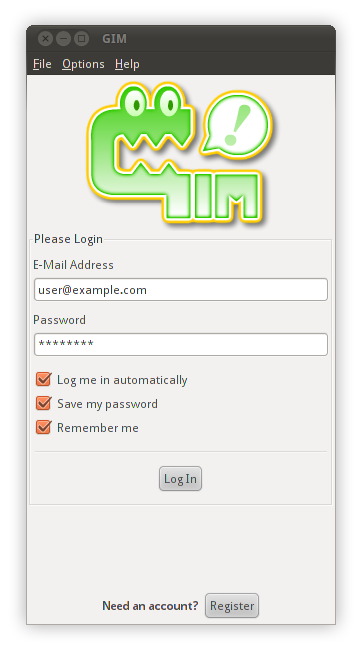
\includegraphics[scale=0.6]{Implementation/diagrams/login.png}
        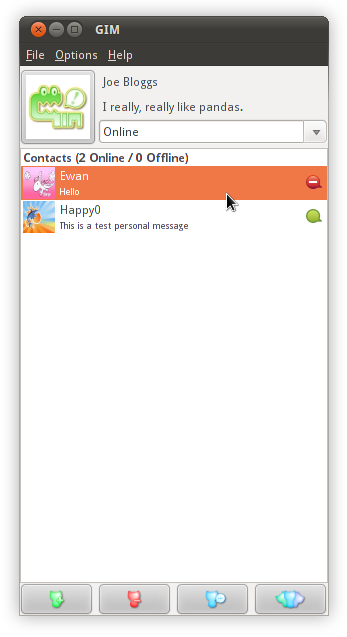
\includegraphics[scale=0.6]{Implementation/diagrams/main.png}
        \caption{The login panel and main window of the GIM Client}
        \label{MainWindowDia}
    \end{center}
\end{figure}

\begin{figure}
    \begin{center}
        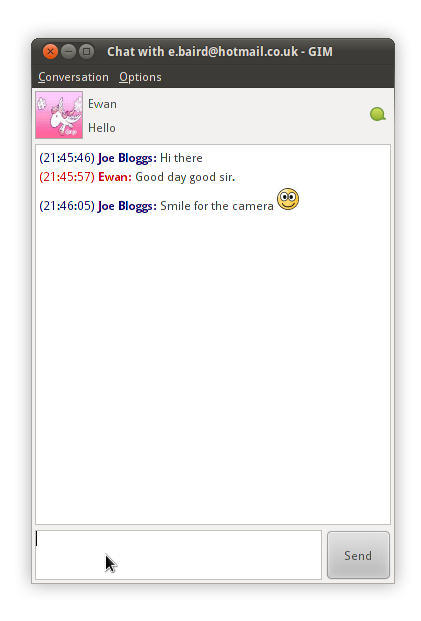
\includegraphics[scale=0.5]{Implementation/diagrams/single_chat.png}
        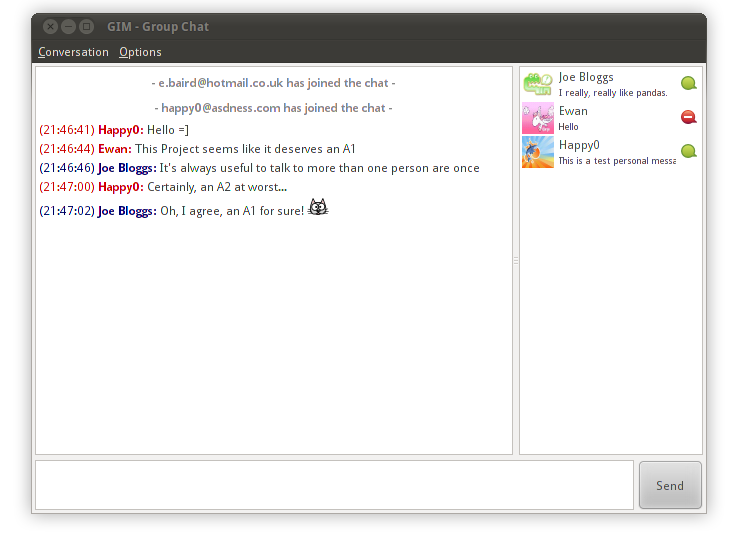
\includegraphics[scale=0.5]{Implementation/diagrams/group_chat.png}
        \caption{Examples of single and group chat windows in GIM.}
        \label{MainWindowDia}
    \end{center}
\end{figure}


\section{Server}

This section will analyse how well the server implementation fulfils the design outlined in section \ref{ServerDesign}. In general, the implementation of the server was a straight-forward affair with very few problems encountered during its development. The most challenging part of the server's development related to concurrency, and is discussed in section \ref{concur}. Spelling errors and typos were the most common cause of problems, however given their easy-to-fix nature, they are not discussed.

\subsection{Concurrency}
\label{concur}
Concurrency was the biggest concern while implementing the server and it was very important that we got it right. Concurrency problems such as race conditions are generally considered to be one of the most difficult problems to debug, so great care was taken to ensure that the possibility of these problems was kept as low as possible. Although we discovered some problems with threading (discussed in section \ref{server_eval}), none of the bugs were caused by race conditions. Instead, confusion about how threads work conceptually caused most of the threading related bugs. For example, in one case an attempt to kill another thread actually caused the current thread to commit suicide. The following describes how thread safety was dealt with and the lessons we learned.

Originally the server used the HashMap class from the \texttt{java.util} package very extensively, primarily because of its very quick look-up times and ability to use user IDs (Strings) as keys. Each User has five HashMaps to store data: their friends, which users have them as a friend, friend requests, blocked users, and rooms they are currently in. Each room uses one to store current users and another to store invited users. The global Data class uses another three to store all of the rooms, users, and workers on the server. This was an issue because HashMaps are not thread-safe, which means each of them had to be wrapped in a synchronised block to ensure thread safety. This was very tedious and very prone to human error. Later on in the development of the server we discovered the \texttt{java.util.concurrent} package, which contains thread-safe implementations of some of the classes in the \texttt{java.util} package, including a thread-safe version of the HashMap class called ConcurrentHashMap. By using the ConcurrentHashMap, it allowed us to remove a lot of the boilerplate code used to make the original implementation thread-safe, and made working with the HashMaps much safer and less prone to human error.

The Buffer class implements a thread-safe, unbounded blocking queue. Essentially the buffer is a LinkedList made thread-safe by only allowing items to be added and removed through synchronised methods. This ensured that at no point could more than one operation be performed on the list, preventing race conditions from occurring.

One of the most difficult to find bugs occurred when a user attempted to log in from 2 different clients. The server located the the worker which was allocated to the client already logged, placed an \texttt{:ERROR:} and \texttt{:QUIT} commands into their buffer, and then set the users worker to the worker of the new client. The new client then mysteriously disconnected. We eventually realised that by putting the \texttt{:QUIT:} command into the workers buffer it was not immediately being disconnected, there would be a slight delay between placing the command into buffer and the command being executed. The \texttt{:QUIT:} command logs out the user and then kills their client. As we had already set the user's worker to the one associated with the new client we were effectively killing both the old and new workers. This was something we had not considered when designing the server. Fortunately the solution was fairly simple and did not require any sizeable changes to the structure of the server. We forced the new worker to wait until the old worker had died, and therefore has empted its buffer and logged the user out, meaning that it was now safe to assign the new worker to the user and log them in.

\subsection{Detecting Abuse and Enforcing Limits}
Originally the server did not enforce any of the limits defined in the protocol and these had to be introduced at a later on in development. As we were aware from the start of development that they would need to be implemented in the future, we were able to design the server so that they could easily be added. 

Limiting the number of commands in moving window turned out to be an interesting problem to solve efficiently.

\begin{verbatim}
this.lastCommandTime = System.currentTimeMillis();
long oldest = this.commandTimes[this.last];

if (oldest != 0 && oldest > (this.lastCommandTime - 5000))
    killWorker();

this.commandTimes[last] = this.lastCommandTime;
this.last = (this.last + 1) % (this.commandTimes.length - 1);
\end{verbatim}


		


\section{Client-Server Communication}
blah blah blah


\section{Storage}
\label{storage}

Both the GIM client and server use Java's built-in serialization features to store data locally while they are not running. The Data class of the server and the Options class of the client both implement Serializable from \texttt{java.io}. This allows them to be serialized and stored on disk using an ObjectOutputStream object (also in \texttt{java.io}).

When the client starts it reads this file from the disk and uses an ObjectInputStream to turn the raw data back into the Options object. For the server, it is not quite so simple. Although the server serializes the entire Data object, some of the data stored in it (such as as rooms) does not need to be persisted across sessions and we create a section Data object and copy the persistent data from the serialized object into it.


\section{Summary}
Despite our problems implementing some of the features, we managed to fix the bugs fairly well. After implementation, things seemed to be working but we needed to do some testing to make sure. The next chapter will describe our testing strategy and some bugs we encountered during the testing.
